\documentclass[a4paper,12pt]{report}
	\usepackage[utf8]{inputenc}
	\usepackage{graphicx}
	\usepackage{hyperref}
	\graphicspath{{figures/}}


\begin{document}
	\title{Virtual Private Networks}
	\author{Bogdan Ionescu}
	\date{\today}
	\maketitle
	\tableofcontents
	
	\chapter{Virtual Private Networks}
	\section{Importance of VPNs}
		In this day and age, networking is everywhere, especially considering the exceedingly fast expansion of the Internet. The Internet, the ultimate network of networks, has radically changed our day-to-day life. Just several years ago, simple everyday habits, such as quickly searching for a piece of information on Google, streaming your favorite songs or paying your bills with just a few clicks would have seemed possible only in a distant future. And yet here we are today, achieving even more impressive tasks, making use of all kinds of networks available within our laptops, phones, tablets and even home electronics, thanks to the IoT.
		
		Unfortunately, the Internet's rapid development also comes with a few important drawbacks which are regrettably often overlooked --- the most significant one being cybersecurity. \textit{Cybersecurity} is the protection of computer systems and networks from the theft and damage of hardware, software or electronic data, as well as from the disruption of the services they provide.\footnote{Wikipedia definition, \url{https://en.wikipedia.org/wiki/Computer_security}} Imagine the consequences if someone managed to obtain all of your credit card information when you are attempting to make an online payment. The damages rise significantly in the case of similar data theft at major companies, which could lead to huge amounts of loss in revenue. In fact, Juniper Research\footnote{\url{https://www.juniperresearch.com/home}} estimates that cybercrime will cost businesses over \$2 trillion in 2019 alone.
		
		Most often, networks are the first obstacle when trying to exploit systems, which is why network security represents such an important key aspect. Surprisingly enough, many protocols used in networking just a few years ago offered no encryption capabilities whatsoever, which led to quite serious vulnerabilities. For example, simple data theft was quite uncomplicated then, when HTTP was predominantly used on the web. Since HTTP alone does not encrypt its data, the communication between our device and a website's server using this protocol would be in cleartext. If someone managed to intercept the network traffic between these two nodes, they would be able to obtain everything that we submit to that website, such as usernames, passwords and even credit card information.
		
		Confidentiality and integrity over networks is also a crucial need for most companies. These usually maintain one or more private networks inside their offices, and only from within these controlled networks employees can access necessary resources. However, these resources must also be available to employees who may be connected to another (possibly also private) network. Such remote access allows employees to work from any part of the world, possibly in case of time-critical emergencies, where response time is vital. This connection must be encrypted in order to prevent traffic sniffing and provide integrity by allowing only authorized users to access the company's private networks. If these conditions are not met, severe breaches often occur, generally leading to a tremendous amount of sensitive data being leaked.
		
	By now you might be thinking how important it is that an application encrypts its data. Unfortunately, sometimes it does not even matter which application we are using! Our outgoing network packets, regardless of what application we are using, will still have our public IPv4 or IPv6 address as a source. Although this may not seem like a serious problem, its implications are quite vast: IP address-based geo-blocking, IP range ban, traffic monitoring etc. These methods represent only a few of those often employed by media companies, governments, intelligence agencies\footnote{\url{https://en.wikipedia.org/wiki/National_Security_Agency\#AT&T_Internet_monitoring}}, or even by countries (The Great Firewall of China\footnote{\url{https://en.wikipedia.org/wiki/Great_Firewall}}).
		
	The question which therefore arises is straightforward and of interest to many of us: how can we achieve confidentiality, integrity and sometimes even anonymity over public networks, such as the Internet? This is where \textit{Virtual Private Networks} (VPNs) prove greatly effective.
		
		\section{What Is a VPN?}
		A Virtual Private Network (VPN) extends a private network by allowing users who are not part of it to send and receive data over a public network, usually the Internet, as if they are directly connected to the private network. VPNs are build using \textit{tunneling protocols}, which establish \textit{tunnels} over public networks, in which the data is encapsulated and most often encrypted\footnote{Encryption is a common, yet not inherent part of VPN connections.}. Classified by the type of topology of connections, VPNs usually are of three types: site-to-site, point-to-point (sometimes also called host-to-host), which are the most common, and a combination of the two, point-to-site.
		
		Site-to-site VPNs establish a tunnel between two networks, thus allowing any authorized host in any of the two networks to make use of it, as shown in figure \ref{fig:site-to-site_VPN}.
		\begin{figure}[h]
			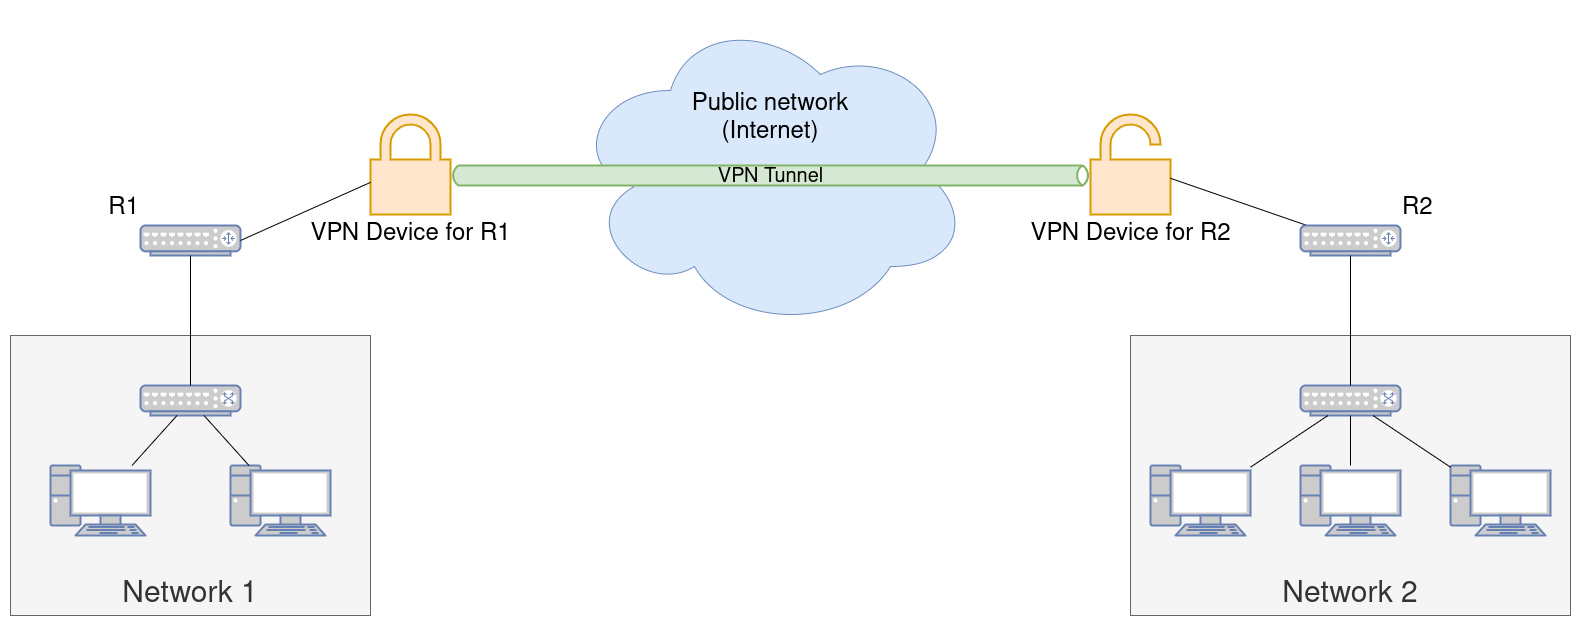
\includegraphics[width=\textwidth]{site-to-site_VPN}
			\centering
			\caption{In this site-to-site architecture, the two VPN devices establish a secure tunnel through the public network. All traffic is encrypted from one site to another. VPN technology can also be directly available in some high-end routers, removing the need for two additional devices.}
			\label{fig:site-to-site_VPN}
		\end{figure}
		
		Advantages of site-to-site VPNs include scalability, being quite straightforward to add another site or device, and high availability, as the VPN tunnel does not depend on a device inside the network to initiate the secure connection (as would be the case with point-to-point architectures), which is why this approach is consistently used by most companies. However, for regular users who wish to remain as private as possible, site-to-site VPNs have a quite serious disadvantage. Since traffic is encapsulated and encrypted just as it leaves the site, by the VPN device or router, data is still vulnerable in the network until it reaches this point, or after it was decrypted, at the other site. As a result, anyone who can intercept our traffic at these stages is a potential threat. Although this scenario is not likely in a company, it is very probable, for example, for someone who wishes to secure his data from a public place which offers free Internet connection, such as a coffee shop or restaurant.
\end{document}